%%%%%%%%%%%%%%%%%%%%%%%%%%%%%%%%%%%%%%%%%%%%%%%%%%%%%%%%%%%%%%%%%%%%%%
% How to use writeLaTeX: 
%
% You edit the source code here on the left, and the preview on the
% right shows you the result within a few seconds.
%
% Bookmark this page and share the URL with your co-authors. They can
% edit at the same time!
%
% You can upload figures, bibliographies, custom classes and
% styles using the files menu.
%
% If you're new to LaTeX, the wikibook is a great place to start:
% http://en.wikibooks.org/wiki/LaTeX
%
%%%%%%%%%%%%%%%%%%%%%%%%%%%%%%%%%%%%%%%%%%%%%%%%%%%%%%%%%%%%%%%%%%%%%%
%
% Template for the American Phytopathological Society's Plant Disease
% Version 1.0 August 2013
%
% Edit the title below to update the display in My Documents
% \title{APS Journal Article}

\documentclass[12pt]{article}

\usepackage[table]{xcolor}
\usepackage{todonotes}
\usepackage{siunitx}
\usepackage{textcomp}
\usepackage{color}

%\DeclareSIUnit{\molar}{M}
%\DeclareSIUnit\molar{\mole\per\cubic\deci\metre}
%\DeclareSIUnit\Molar{\textsc{m}}
%\DeclareSIUnit[number-unit-product = {}]\degree{\SIUnitSymbolDegree}

% Text layout
\topmargin 0.0cm
\oddsidemargin 0.5cm
\evensidemargin 0.5cm
\textwidth 16cm 
\textheight 21cm


% Handles the footer
\usepackage{fancyhdr}
\pagestyle{fancy}

\fancyhf{} % delete current header and footer
%\fancyhead[LE,RO]{\bfseries\thepage}
\renewcommand{\headrulewidth}{0pt}
\renewcommand{\footrulewidth}{1pt}
%\addtolength{\footheight}{0.5pt} % space for the rule
%\addtolength{\headheight}{0.5pt} % space for the rule
\fancyfoot[LO]{Knaus, Fieland, and Gr\"{u}nwald}
\fancyfoot[CO]{\thepage}
\fancyfoot[RO]{\emph{Plant Disease}}

%\fancyfoot[CO]{
%\noindent\makebox[\linewidth]{\rule{\textwidth}{1pt}}
%Knaus \vspace{20mm} \thepage \vspace{80mm} \emph{Plant Disease}
%}

% amsmath package, useful for mathematical formulas
\usepackage{amsmath}
% amssymb package, useful for mathematical symbols
\usepackage{amssymb}

% graphicx package, useful for including eps and pdf graphics
% include graphics with the command \includegraphics
\usepackage{graphicx}

% cite package, to clean up citations in the main text. Do not remove.
\usepackage{cite}
\renewcommand\citeleft{(}
\renewcommand\citeright{)}

%\usepackage{color} 

%enable umlaut, etc.
\usepackage[utf8]{inputenc}

% Use doublespacing - comment out for single spacing
%\usepackage{setspace} 
%\doublespacing

% Text layout
%\topmargin 0.0cm
%\oddsidemargin 0.5cm
%\evensidemargin 0.5cm
%\textwidth 16cm 
%\textheight 21cm

% Bold the 'Figure #' in the caption and separate it with a period
% Captions will be left justified
\usepackage[labelfont=bf,labelsep=period,justification=raggedright]{caption}

% Change Figure to Fig.
\renewcommand{\figurename}{Fig.}


% Define orange for highlighting text (NIK)
\definecolor{orange}{rgb}{1,0.5,0}

% Use the PLoS provided bibtex style
%\bibliographystyle{plos2009}

% Use the American Phytopathological Society's bibtex style
% Details can be found at: http://apsjournals.apsnet.org/userimages/ContentEditor/1236780011229/pd_author_instructions.pdf
\bibliographystyle{amphs}

% Remove brackets from numbering in List of References
\makeatletter
\renewcommand{\@biblabel}[1]{\quad#1.}
\makeatother

% Leave date blank
\date{}



%\pagestyle{myheadings}
%% ** EDIT HERE **
\usepackage{lineno}

%% ** EDIT HERE **
%% PLEASE INCLUDE ALL MACROS BELOW

%% END MACROS SECTION

\begin{document}

%\renewcommand\@seccntformat[]{}

Checklist for success!

\begin{enumerate}
  \item Fasta of sequences used for PCR RFLP development or accessions.
  \item Table of PCR RFLP fragment sizes.
  \item \emph{P. syringae} (1909), \emph{P. plurivora} (2009) and \emph{P. pini} (2011) as most abundant in our study.
%\emph{P. hibernalis} (1925)
%  \item The third etc \ldots
\end{enumerate}

\newpage


% Title must be 150 characters or less
\begin{flushleft}
{\large
\textbf{Diversity of foliar \textit{Phytophthora} species on \textit{Rhododendron} in Oregon nurseries}
}
\\

\hspace{12pt}

\textbf{B. J. Knaus,} Horticultural Crop Research Unit, USDA-ARS, Corvallis, OR 97330; \textbf{V. Fieland,} Department of Botany and Plant Pathology, Oregon State University, Corvallis, OR 97331; and \textbf{N. J. Gr\"{u}nwald,} Horticultural Crop Research Unit, USDA-ARS\\

\end{flushleft}

%\hspace{12pt}

\noindent\makebox[\linewidth]{\rule{\textwidth}{1pt}} 

% Please limit the abstract to 200 words in one paragraph
\section*{\sffamily\normalsize\centerline{Abstract}}

%\begin{abstract}

% Insert Author names, affiliations and corresponding author email.
\begin{flushleft}
Knaus, B. J., Fieland, V., and Gr\"{u}nwald, N. J. 20XX. Diversity of foliar \textit{Phytophthora} species on \textit{Rhododendron} in Oregon nurseries. Plant Dis. XX:XXX-XXX.
\\

\hspace{12pt}


% Please keep the abstract between 250 and 300 words
%\section*{Abstract}
\linenumbers

%\todo[color=orange!40, inline]{What is this paper about?}

The genus \emph{Phytophthora} is considered to contain some of the most important plant pathogens affecting nursery crops. Given the recent emergence of the sudden oak death pathogen \emph{P. ramorum}, particularly in association with \emph{Rhododendron}, it becomes prudent to characterize \emph{Phytophthora} communities in nursery environments.  Many taxa may present syptoms similar to regulated taxa and may vary in pathogenicity from regulated taxa.  We present a survey of \emph{Phytophthora} taxa observed from nine nurseries in the U.S. state of Oregon.  Incidence and diversity of \emph{Phytophthora} communities differed significantly among nurseries and among seasons.  The taxa \emph{P. syringae} and \emph{P. plurivora} were widespread and detected at most of the nurseries sampled.  Nine other taxa were also detected but were found either in a single nursery or were shared among only a few nurseries.  Charactertization of the \emph{Phytophthora} communities present in nurseries is an important step towards understanding the ecology of these organisms as well as an aid to nursery managers in determining what risks may be present when symptomatic plants are observed.  This study builds on an increasing literature which characterize \emph{Phytophthora} community structure in nurseries.


\hspace{12pt}

Corresponding author: N. J. Gr\"{u}nwald; E-mail: grunwaln@science.oregonstate.edu.

\end{flushleft}

%\end{abstract}

\noindent\makebox[\linewidth]{\rule{\textwidth}{1pt}} 


%\hspace{12pt}

% Please keep the Author Summary between 150 and 200 words
% Use first person. PLoS ONE authors please skip this step. 
% Author Summary not valid for PLoS ONE submissions.   
%\section*{Author Summary}

%\section*{Introduction}
\section*{} % Introduction section title omitted in APS style

\linenumbers

%\todo[color=green!40, inline]{Cature the paper in a few sentences.  Abstract too.}

The greenhouse and nursery industry in the US state of Oregon is perhaps the most important agricultural industry in the state.  During 2011 its worth was \$742 million USD down from ca. \$1 billion in 2007 \cite{oda_2012}.  This represented 14\% of the state's agricultural production in 2011.  Management and mitigation of plant pathogens to this industry therefore presents an important role in the state's economy.  A fundamental task in this management and mitigation is characterization of the plant pathogens present in these nurseries in order to develop best managmenet practices and critical control points for implementation of systems approaches\cite{parke_grunwald_2012}.

The plant pathogens in the genus \emph{Phytophthora} play an important role in the nursery industry. The nursery industry was severly impacted by the recent emergence of the sudden oak death pathogen \emph{P. ramorum} due to the fact that this pathogen is subject to federal quarantine \cite{werres_etal_2001,grunwald_etal_2008}.  Export of host plant taxa among states in the USA is regulated to prevent further spread of this pathogen.  The sudden oak death pathogen has a broad host range including many taxa important to the nursery industry \cite{tooley_etal_2004, hansen_etal_2005}.  It is now evident that \emph{P. ramorum} emerged at least 3 times in the US and 5 times globally \cite{grunwald_etal_2012,van_poucke_etal_2012}. \emph{P. ramorum} is primarily a foliar pathogen on nursery crops such as \emph{Rhododendron}, \emph{Camellia}, and \emph{Pieris}. However, determining whether lesions observed at a particular location may be attributable to the quarantined \emph{P. ramorum} or any of the non-quarantined species of \emph{Phytophthora} presents a challenge.  Thus, understanding of the community of foliar infecting \emph{Phytophthora} taxa present in nurseries represents an important first step in development and implementation of best management practices.

Here we present a survey of \emph{Phytophthora} communities present on \emph{Rhododendron} in nine commercial nurseries located in the US state of Oregon.  Directed searches were performed to attempt to identify symptomatic \emph{Rhododendron} plants, that is, plants possessing leaves with lesions characteristic of foliar \emph{Phytophthora} infection.  These putatively infected samples were validated using growth on selective media and DNA based tools to confirm their identity.  In order to ease the molecular screenning for nursery \emph{Phytophthoras} an amplicon restriction based assay was developed to determine \emph{Phytophthora} taxa.  Six of the nurseries were sampled during two different seasons (fall and spring), while three were only sampled once (both in the spring).  We used these data to test the hypothesis that \emph{Phytophthora} communities in \emph{Rhododendron} nurseries in Oregon differ significantly among nursery as well as season.
%A secondary objective was development of a restriction assay useful in rapid and cost effective identification of \emph{Phytophthora} species infecting \emph{Rhododendron}.

%%%%% ----- Section ----- %%%%%

\section*{\sffamily\normalsize{Materials and Methods}}

\todo[color=green!40, inline]{Val questioned whether this should be seven nurseries. We did summarize all nine, so I think this number should be presented.  Also, six and not seven appear to have been sampled during two seasons.}

\textbf{Sampling strategy.} \emph{Phytophthora} species were systematically sampled focusing on symptomatic lesions observed in contiguous blocks of \emph{Rhododendron} plants in commercial nurseries.  A total of nine nurseries were sampled, seven of of which were sampled in both  the spring and fall.  These nurseries represent a majority of Oregon counties in the Willamette Valley (Fig. \ref{fig:map}).  Two sites were sampled within each nursery.  Each site typically consisted of one greenhouse, hoophouse or other group of contiguous \emph{Rhododendron} plants.  Within each site, three blocks of \emph{Rhododendron} plants were sampled following a zig-zag pattern through each block.  Sampled plants were spaced by three to six meters when possible.  Three to four leaves were collected from each of approximately 20 symptomatic plants.

\textbf{Taxonomic validation based on selective media.} In order to validate that collected leaves contained \emph{Phytophthora} lesions, leaves were plated on selective media.  Symptomatic leaves were collected from each nursery and stored at room temperature overnight.  Leaves were surface sterilized by washing in a 2\% household bleach solution with a subsequent rinse in deionized water.  A flame sterilized paper hole punch was used to cut five to eight disks from the leading edge of growth of leaf lesions.  Disks were embeded in the \emph{Phytophthora} selective media PARP (20\% filtered V8 juice; 100 ppm PCNB; 250 ppm sodium ampicillin; 10 ppm rifampicin; 10 ppm pimaricin)\cite{jeffers_martin_1986} and incubated at 20$^\circ$C until growth was observed (typically 5-7 days).  A plug from the leading edge of these cultures was subcultured on PARP selective media to obtain a clean culture.

\textbf{Taxonomic validation based on genotyping.} Genetic validation of isolates was performed by either restriction fragmentation (PCR-RFLP) of the PCR amplified internal transcribed spacer of the ribosomal DNA (ITS) or restriction combined with sequencing of ITS.  Aerial hyphae were collected from the surface of cultured isolates using a sterile toothpick and transferred to \SI{100}{\micro\liter} deionized water.  The hyphae containing water solution was boiled for five minutes at 95.9$^\circ$C on a ABI 9700 or Veriti thermocycler (Applied Biosystems, Foster City, CA).  Polymerase chain reaction was performed using \SI{5}{\micro\liter} of the boiled hyphal mixture, 1.5 mM MgCl$_{2}$, 0.2 mM of each dNTP, 0.4 mM of primers ITS4 and ITS6 \cite{grunwald_etal_2011, cooke_etal_2000}, \todo[color=green!40]{Is this correct? Needs to be units, not conc.} 1.25 U $Taq$ polymerase (Genscript Corporation, Piscataway, NJ) and molecular grade water to attain a final volume of \SI{25}{\micro\liter}.  The reaction was performed with an initial denaturation at \SI{94}{\celsius} for 3 minutes followed by 35 cycles consisting of one minute annealing at \SI{54}{\celsius}, one minute extension at \SI{72}{\celsius} and one minute denaturation at \SI{94}{\celsius}.  A final extension step was performed at \SI{72}{\celsius} for 10 minutes.

\todo[color=orange!40, inline]{Should our `known' strains be documented? If they were from NCBI maybe we just need accessions.}

To aid \emph{Phytophthora} identification an amplicon restriction assay was developed.  The restriction assay was designed using \emph{Phytophthora} ITS sequences from the National Center for Biotechnology Information (NCBI; http://www.ncbi.nlm.nih.gov/).  These sequences were queried using the software Geneious (Biomatters Inc., San Francisco, CA) for a restriction enzyme which would produce a diagnostic fingerprint assay.  This assay was then implemented on our nursery samples.  Restriction of ITS amplicons was performed with the enzyme \emph{Aci}I according to manufacturer's directions (New England Biolabs, Ipswich, MA).  Digested DNA was fingerprinted on a 2\% agarose gel (w/v) with a 1kb-plus ladder (Life Technologies, Grand Island, NY) run in 1X TAE buffer for 2.0 hours at 60V.  When an unexpected fragement pattern was observed, the amplified ITS locus was sequenced.  Approximately 20\% of the isolates with expected fragment patterns were also sequenced for quality control purposes.  Sequencing was performed at the Oregon State University's Center for Genome Research and Biology using ABI's Big Dye Terminator chemistry and sequenced on an ABI 3730 capillary sequencing machine (Applied Biosystems Inc., Foster City, CA).  Sequences were identified to species using Phytophthora-ID \cite{grunwald_etal_2011}, a web-based blast \cite{altschul_etal_1990} tool with a \emph{Phytophthora} specific database.  Samples which shared greater than a 99\% sequence identity were considered matches while samples with less than 99\% sequence identity were identified to the most similar species and given a `-like' designation.

\todo[color=orange!40, inline]{Need a fasta of sequences for figshare? Not if they're all accessioned though.}

\textbf{Statistical analyses.} A map of Oregon counties sampled was created with the R package Maps in S \cite{R, r_maps}.  Summaries of nursery diversity were calculated in the R package vegan \cite{R, vegan}.  These included the sample size, richness (number of species), Shannon-Wiener index, evenness (the Shannon-Wiener index divided by it's maximum expected value in order to scale it from zero to one) and Simpson's index (i.e., the probability that two individuals sampled at random will be of different species).

In order to address the hypotheses of whether diversity is evenly partitioned among nurseries, as well as among seasons within nurseries, we used additive diversity partitioning as implemented in the R package vegan \cite{vegan} and discussed in \cite{lande_1996, christ_etal_2003}.  This analysis can be seen as an ANOVA analog where a diversity metric is used as the dependent variable.  Among group diversity ($\beta$-diversity) can be derived from within group diversity ($\alpha$-diversity) subtracted from total diversity ($\gamma$-diversity).  This can be made hierarchical by using $\alpha$-diversity at the next highest level as $\gamma$-diversity for that level.  We used nursery and among season, within nursery as two hierarchcal levels.  In order to correct for a potentially unbalanced sample we used diversity estimates weighted by their proportionality.  To test for significance we randomly assigned diversity among the categories and derived our diversity estimates again, repeating this for a total of 999 times.  Because nurseries B, C and G \todo[color=orange!40]{Nursery G was only sampled in spring 3/19/12, right?} were only sampled during one season (Table \ref{tab:sample}), they were omitted from this analysis.

%%%%% ----- Section ----- %%%%%

\section*{\sffamily\normalsize{Results}}

A total of nine nurseries were sampled during 2011 and 2012 (Fig. \ref{fig:map}, Table \ref{tab:sample}).  Of these nurseries, six were visited during two seasons while three nurseries were sampled during one season (Table \ref{tab:sample}).  From these nurseries, a total of 438 isolates were obtained across all locations and dates.  Isolates were identified to species using PCR-RFLP and sequencing of the ITS region. A total of 11 taxa were observed in 438 samples (Table \ref{tab:taxa_counts}).

An assay based on restriction digestion of PCR amplicons of the ITS region was developed.  A total of \textcolor{red}{999} sequences from \textcolor{red}{12} \emph{Phytophthora} taxa were obtained from NCBI and queried for restriction enzyme fragment patterns.  This resulted in the enzyme \emph{Aci}I being chosen as the most highly diagnostic enzyme (Fig. \ref{fig:gel}).  The taxa \emph{P. hibernalis}, \emph{P. parsiana}, \emph{P. plurivora} and taxon Pgchlamydo each produced a single banding pattern which was unique to each taxon.  Digestion of \emph{P. syringae} samples resulted in four banding patterns.  Three of these were the product of a codominant C/T transversion while the fourth remains uncharacterized.  All four of these fingerprints were unique to \emph{P. syringae}.  Several other taxa shared banding patterns which were unique to a small set of taxa but distinguished this small set from the other taxa.  \emph{P. pini} and \emph{P. citricola} III shared a banding pattern which allowed for identification that a sample was one of these two taxa, but could not distinguish among these two taxa.  \emph{P. hedraiandra} and \emph{P. cactorum} shared a banding pattern which was unique to these two taxa but invariable between them.  A single banding pattern was shared by \emph{P. bilorbang}, \emph{P. lacustris} and \emph{P. riparia}.  This assay provides for rapid diagnostics for many taxa encountered in Oregon nursery environments.

%\todo[color=red, inline]{Is hedraiandra spelled correctly?}


\todo[color=orange!40, inline]{Need a paragraph on the PCR-RFLP assay.  Should fragment size be reported in text or in a table?  Brian's vote = table.}

%The PCR-RFLP assay was validated by resequencing \colorbox{orange}{XX} isolates after PCR. All isolates could be unabiguously identified using the PCR RFLP assay described in the previous section. Typical digests are shown in Fig. \ref{fig:gel}. \colorbox{orange}{figure 2}\todo[color=yellow!80]{Val, add nice gel images as discussed}).

Incidence and abundance of foliar \emph{Phytophthora} varied dramatically among nursery as well as among season for each nursery (Fig. \ref{fig:nursdiv}).  The most abundant taxon was \emph{P. syringae}, which was observed in every nursery at almost every season (Table \ref{tab:taxa_counts}).  While it was abundant in nurseries A, B, F and I, it was rare in nurseries E and G.  The second most abundant taxon, \emph{P. plurivora}, was abundant in nursery E, moderately abundant in nurseries A, D, H and I, but absent from nurseries C and G.  The third most abundant taxon, \emph{P. hibernalis}, occured at relatively high abundance in nursery D, but did not occur in the other nurseries.  The remaining taxa were relatively rare.

Diversity of foliar \emph{Phytophthora} communities within each nursery varied dramatically.  Shannon-Weiner indicies ranged from 0.124 to 1.587 while evenness ranged from 0.179 to 0.874 (for samples with more than one observed taxon; Table \ref{tab:div}).  This represented a range of close to 70\% of its theoretical range.  Similarly, Simpson's index demonstrated a broad range of values ranging from 0.053 to 0.750 (Table \ref{tab:div}).  Because Simpson's index is a probability, it ranges from zero to one.  The range of Simpson's indices observed in Table \ref{tab:div} includes almost the entire theoretical range of this index.  Differences among season for certain nurseries was evident as well.  For example, nurseries D and I demonstrated large differences in diversity among spring and fall.  However, nurseries A and H demonstrated relatively consistent diversities among seasons.  It is also noteworthy that abundance is not necessarily correlated with diversity.  Nursery E had a moderate number of isolates (58 isolates), but one of the lowest diversities (Table \ref{tab:div}).  Nursery G had a low number of isolates detected, but demonstrated a relatively high diversity.  However, nursery D did have the largest number of isolates detected and demonstrated a relatively high diversity, therefore complying with the idea that abundance may contribute to diversity.

Differences in diversities among nurseries and among seasons within nurseries were statistically significant (Table \ref{tab:adipart}).  Total diversity was not statistically significant because this category encompasses the entire sample, such that re-assigning isolates to other groupings does not affect this estimate.  Within nursery diversities were statistically significant with a negative z-value, indicating less observed diversity in our sample relative to a sample assuming a uniform distribution of diversity (Table \ref{tab:adipart}).  This pattern is likely driven by nurseries H and I which have a relatively large amount of diversity as well as nurseries A and E which had relatively low diversity (Table \ref{tab:div}).  Differences in diversity among nurseries (Table \ref{tab:adipart}) were similarly significant.  Differences in diversities among seasons, within nurseries were also significant (Table \ref{tab:adipart}).  Nurseries D, F and I had the greatest differences in diversity among seasons (Table \ref{tab:div}).  Note that while isolate number for nursery I was similar among seasons (Table \ref{tab:adipart}, Fig. \ref{fig:nursdiv}) the diversity in spring was much less than in the fall.  Nurseries A and E showed relatively little change in diversity among seasons (Table \ref{tab:div}).  Again, noting that for nursery E, abundance changed dramatically (Fig. \ref{fig:nursdiv}) but the diversity estimates were very similar (Table \ref{tab:div}).  The majortity of the diversity within the \emph{Phytophthora} nurseries sampled was contained within seasons and nurseries while among nursery diversity accounted for the second greatest component (Fig. \ref{fig:propdiv}).

%\subsection*{Subsection 1}

%\subsection*{Subsection 2}

%%%%% ----- Section ----- %%%%%

\section*{\sffamily\normalsize{Discussion}}

%Sampling of nine Oregon \emph{Rhododendron} nurseries resulted in a total of 438 isolates representing 11 species of \emph{Phytophthora}.  The most commonly observed taxa were \emph{P. syringae} followed by \emph{P. plurivora} and \emph{P. hibernalis}.  While the first two were common among sampled nurseries in Oregon, the abundance of \emph{P. hibernalis} was attributable to one nursery (Fig. \ref{fig:nursdiv}).  The remaining eight taxa represent rare taxa which were ephemerally observed in a small number of nurseries.  Our sample suggests that Oregon \emph{Rhododendron} nurseries will typically have \emph{P. syringae} and perhaps \emph{P. plurivora} while also including a few rare taxa which may be specific to a nursery.

Characterizing the \emph{Phytophthora} communities in nurseries represents an important first step in management of these pathogens.  Some taxa, such as \emph{P. ramorum}, are quarantined and may represent a significant financial burden to a nursery when discovered.  Other taxa may create symptoms similar to regulated taxa, but not be on a list of quarantine species, making it important to distinguish the taxa which lead to symptomatic plants.  Similarly, some taxa may create lesions, but lack the pathogenicity or dispersal capabilities of other taxa, making their presence benign.  Understanding the communities of \emph{Phytophthora} in nurseries builds an expectation and provides initial information for managing their presence.

We found that \emph{Phytophthora} communities in Oregon nurseries differed significantly among nursery as well as among season within nurseries (Table \ref{tab:adipart}).  This indicates that on any visit to any nursery one may expect to encounter a different constituency of \emph{Phytophthora} taxa, even on visits to the same nursery but during different times of the year (Fig. \ref{fig:nursdiv}).  For example, visits to nursery D resulted in a high frequency of \emph{P. hibernalis} observation (Table \ref{tab:taxa_counts}; Fig. \ref{fig:nursdiv}), a finding not observed in the other nurseries.  Similarly, a visit to nursery F in the fall may result in a high abundance of \emph{P. pini}/\emph{P. citricola} III while a visit in spring may result in a high abundance of \emph{P. syringae}.  Despite these marked differences some generalizations can be made.  The most abundant taxon was \emph{P. syringae} which was observed in every sampled nursery (Table \ref{tab:taxa_counts}).  Similarly, \emph{P. plurivora} was observed in almost every nursery (Table \ref{tab:taxa_counts}).  The third most commonly observed taxon, \emph{P. pini}/\emph{P. citricola} III was observed in moderate abundance, but only at three of the nine nurseries (Table 2).  The quarantined taxon, \emph{P. ramorum}, was not observed in any of the sampled nurseries.  This suggests that any leaf lesion observed in an Oregon nursery which appears to be due to a \emph{Phytophthora} infection is likely to not be \emph{P. ramorum} and that \emph{P. syringae} and \emph{P. plurivora} are more likely candidates.

%Our results appear congruent with other reports from \emph{Phytophthora} surveys in North America.

Results reported by other groups share some features in common with our work, but also highlight the heterogeneity of \emph{Phytophthora} taxa found in nurseries.  Some comparisons are not straight forward due to recent nomenclatural changes where the taxon \emph{P. citricola} has been divided into \emph{P. citricola} III, \emph{P. multivora}, \emph{P. plurivora}\cite{jung_burgess_2009} and \emph{P. pini}\cite{hong2011}.  Schwingle et al.\cite{schwingle_etal_2007} surveyed 45 Minnesota nurseries in 2002 and 2003 and found five \emph{Phytophthora} taxa found on \emph{Rhododendron} leaves with \emph{P. cactorum} to as the most abundant followed by \emph{P. citricola} and \emph{P. citrophthora}.  They further reported surveys from 12 Minnesota nurseries in 2004 and 10 nurseries in 2005 where they found five \emph{Phytophthora} taxa on \emph{Rhododendron} with \emph{P. citricola} the most abundant and the others rare.  Warfield et al. surveyed 14 nurseries in North Carolina during 2003 \cite{warfield_etal_2008}.  They detected three species of \emph{Phytophthora} on \emph{Rhododendron} and found \emph{P. citricola} and \emph{P. cambivora} to be the most abundant while \emph{P. cactorum} was rare.  Donahoo and Lamour surveyed 29 Tennessee nurseries during 2004 and 2005\cite{donahoo_lamour_2008}.  They detected seven \emph{Phytophthora} taxa with \emph{P. citricola} as the most frequently isolated \emph{Phytophthora} derived from \emph{Rhododendron} leaves with \emph{P. citrophthora} and \emph{P. nicotianae} as second and third most common.  Yakabe et al. reported \emph{Phytophthora} taxa recovered from leaf samples from 1,619 nurseries in California during 2005 and 2006 \cite{yakabe_etal_2009}.  They observed eight \emph{Phytophthora} taxa on \emph{Rhododendron} (including \emph{Azalea}) with \emph{P. citricola}, \emph{P. foliorum} and \emph{P. syringae} as similarly abundant with the remaining taxa being relatively rare.  Bienapfl and Balci \cite{bienapfl_balci_2013} surveyed 10 Maryland nurseries over a three year period (2010-2011).  Their survey not only included samples from each nursery but included samples which had recently arrived at the nurseries, typically from West Coast suppliers.  They reported the detection of ten \emph{Phytophthora} taxa associated with \emph{Rhododendron} with \emph{P. cinnamomi}, \emph{P. citrophthora}, \emph{P. pini}, \emph{P. plurivora} and \emph{P. multivora} as being abundant and the remaining taxa relatively rare.  Among plants which had recently been shipped to Maryland nurseries they detected six \emph{Phytophthora} taxa associated with \emph{Rhododendron} with \emph{P. plurivora}, \emph{P. pini} and \emph{P. citrophthora} being abundant and the remaining taxa as rare.  Common to all these reports is the presence of taxa within the \emph{P. citricola} complex.  While \emph{P.syringae} was common in our surveys the only other report to find this taxon as abundant was the other U.S. west coast report of Yakabe et al. \cite{yakabe_etal_2009}.  Perhaps the most notable omission in our report was \emph{P. citrophthora} which was frequently abundant in other surveys but absent in ours.


%as the most abundant \emph{Phytophthora} recovered from \emph{Rhododendron} leaves (including \emph{Azalea}) followed by \emph{P. foliorum}, \emph{P. syringae} and \emph{P. citrophthora}.

\todo[color=orange!40, inline]{Omitted Leonberger et al., doesn't provide information to subset host to Rhodo!}
% 
%  \item[Leonberger] Leonberger et al. \cite{leonberger_etal_2013} surveyed nurseries, greenhouses and landscapes of Iowa, Michigan and Indiana during the years 2006 to 2008.  They report collecting 121 \emph{Phytophthora} isolates from 32 genera of hosts.  The most commonly observed \emph{Phytophthora} taxa in their sample was \emph{P. citricola} followed by \emph{P. citrophthora}, \emph{P. nicotianae} and \emph{P. cactorum}.  Of relevance to the present study, they did observe \emph{P. syringae} but at low abundance.







%While \emph{P. citricola} was reported frequently in the above literature, its taxonomic status is in a state of change \cite{jung_burgess_2009, hong2011}.

%Olson and Benson \cite{olson_benson_2011}.
%Olson et al. \cite{olson_etal_2013}.

A characterization of the \emph{Phytophthora} communities present in nurseries represents important first steps in implementing knowledge based management systems.  Current methods for identification of \emph{Phytophthora} in nurseries consists of culturing on selective media \cite{jeffers_martin_1986} or an enzyme-linked immunosorbent assay (i.e., ELISA) test.  These tests typically validate whether a sample can be attributed to an organism in the genus \emph{Phytophthora}, but does not diagnose the species.  Determination at the species level typically requires more expensive molecular genetic tools \cite{grunwald_etal_2011} and typically are developed to address only taxa which are legally regulated (e.g., \emph{P. ramorum} and \emph{P. infestans}).  Knowledge of the species contributing to a community of \emph{Phytophthora} may therefore not only aid in species specific management strategies, but may help researchers prioritize which taxa to focus on during efforts to develop cost effective marker systems.  Our research demostrates a great amount of heterogeneity among Oregon nurseries.  While some taxa appear ubiquitous (i.e., \emph{P. syringae} and \emph{P. plurivora}), much of the observed diversity is localized to one or a few nurrseries.  This suggests that as more nurseries are surveyed, a greater amount of \emph{Phytophthora} diversity may be discovered.  This work marks an important step toward characterizing \emph{Phytophthora} communities in nurseries and sets a foundation for future studies which, if similar to the results presented here, will continue to reveal novel features of \emph{Phytophthora} community structure.



%  Now that we have begun to characterize the communities of foliar \emph{Phytophthora} present in our nurseries we can plan strategies to mitigate specific taxa.


%\todo[color=green!40, inline]{Hmm, did I go out strong or with a whimper?}

% Do NOT remove this, even if you are not including acknowledgments
\section*{\sffamily\normalsize{Acknowledgments}}
This project was supported by funds from USDA-ARS CRIS Project 5358-22000-039-00D, the USDA-ARS Floriculture Nursery Initiative, and the Oregon Department of Agriculture/Oregon Association of Nurseries (ODA-OAN) research programs. We thank Karan Fairchild, Meg Larsen, Caroline Press and Kimberly Bellingham for technical and administrative support. 

%\section*{Literature Cited}
% The bibtex filename
\renewcommand\refname{Literature Cited}
\bibliography{foliar_thora}

\clearpage

\section*{Figure Legends}
% Figures are either 85 mm wide (one column) or
% 178mm wide (two columns).



%\begin{figure}[!ht]
%\begin{center}
%%\includegraphics[width=4in]{figure_name.2.png}
%\end{center}
%\caption{
%{\bf Bold the first sentence.}  Rest of figure 2  caption.  Caption 
%should be left justified, as specified by the options to the caption 
%package.
%}
%\label{Figure_label}
%\end{figure}



\begin{figure}[!ht]
\begin{center}
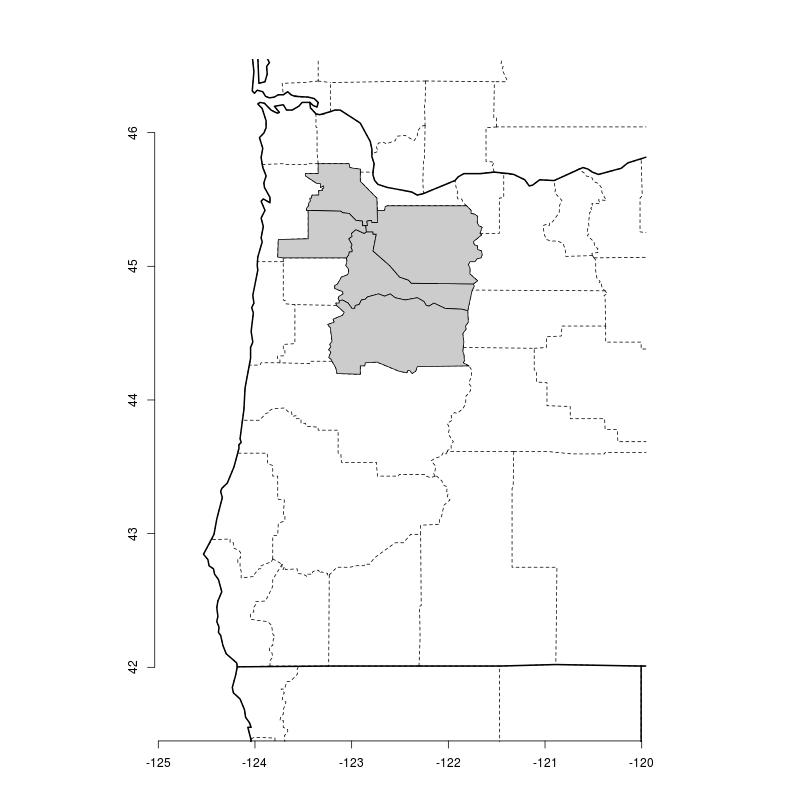
\includegraphics[width=85mm, height=85mm]{../rstuff/nursmap.png}
\end{center}
\caption{
Map of Oregon counties containing nurseries sampled for \emph{Phytophthora} community structure (see Table \ref{tab:sample}).
%%should be left justified, as specified by the options to the caption 
%package.
}
\label{fig:map}
\end{figure}
\clearpage

\begin{figure}[!ht]
\begin{center}
\includegraphics[width=178mm, height=85mm]{../figure_rflp/fig2.pdf}
%\missingfigure[figwidth=6cm]{Gel of PCR RFLP}
\end{center}
\caption{
Gel image demonstrating diagnostic differences among \emph{Phytophthora} taxa. PCR amplicons of the internal transcribed spacer region were digested with the enzyme \emph{Aci}I and resolved on a 2\% agarose gel.  A 1kb-plus DNA ladder is shown in lanes 1 and 18.  The size of bands in this ladder, in base pairs, for select fragments is presented to the left of lane one.  Brackets indicate taxa which cannot be differentiated based on this assay.  The ITS region was sequenced for these samples to determine their identity.
%%should be left justified, as specified by the options to the caption 
%package.
}
\label{fig:gel}
\end{figure}
%\todo[color=green!40, inline]{I guessed at most of this.  Can Val correct this?}
\clearpage




\begin{figure}[!ht]
\begin{center}
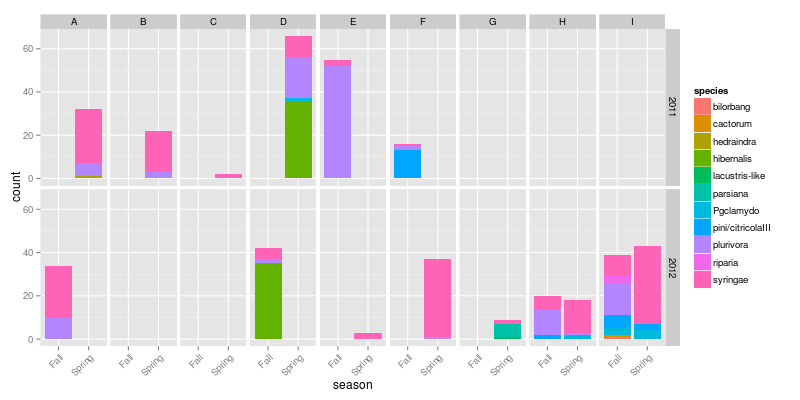
\includegraphics[width=178mm,height=85mm]{../rstuff/nursdiv.png}
\end{center}
\caption{
Barplot of \emph{Phytophthora} species incidence.  Nurseries (A-I) are in columns with season (fall and spring) in subcolumns.  Year sampled is presented in rows.
%%should be left justified, as specified by the options to the caption 
%package.
}
\label{fig:nursdiv}
\end{figure}
\clearpage

\begin{figure}[!ht]
\begin{center}
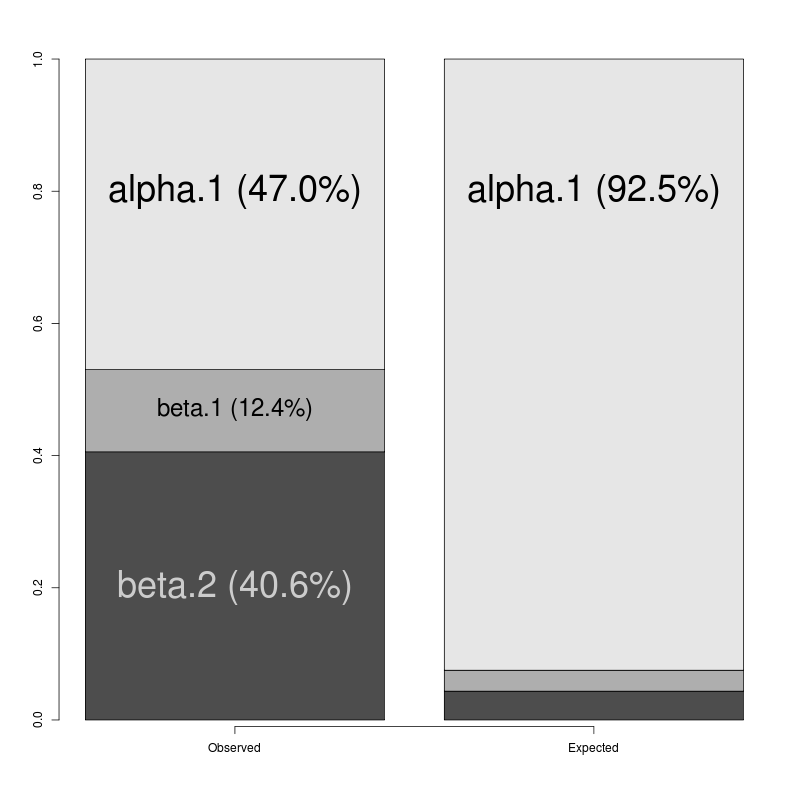
\includegraphics[width=85mm, height=85mm]{../rstuff/propdiv.png}
\end{center}
\caption{
{\bf Barplot of diversity proportions.} Most of the diversity was partitioned within nurseries (alpha.1) resulting in a high amount of among nursery diversity differences (beta.2).
%%should be left justified, as specified by the options to the caption 
%package.
}
\label{fig:propdiv}
\end{figure}
\clearpage

\section*{Tables}
%\begin{table}[!ht]
%\caption{
%\bf{Table title}}
%\begin{tabular}{|c|c|c|}
%table information
%\end{tabular}
%\begin{flushleft}Table caption
%\end{flushleft}
%\label{tab:label}
% \end{table}

\begin{table}[!ht]
\caption{Sample and date of nurseries.  The sampling goal was to visit each nursery during both spring and fall.  The month of each visit is presented in the cell for each date and nursery visit.}
\begin{tabular}{cccccc}
\hline
\textbf{Nursery} & \textbf{County} & \textbf{Spring 2011} & \textbf{Fall 2011} & \textbf{Spring 2012} & \textbf{Fall 2012} \\
\hline
A & Washington & March & & & December \\
D & Yamhill & April & & & November \\
E & Clackamas & & November & April & \\
F & Marion & & November & March & \\
H & Clackamas & & & March & November \\
I & Linn & & & April & December \\
B & Marion & March & & & \\
C & Clackamas & April & & & \\
G & Marion & &  & March & \\
\hline
\end{tabular}
%\begin{flushleft}Table caption
%\end{flushleft}
\label{tab:sample}
\end{table}


% latex table generated in R 3.0.2 by xtable 1.7-1 package
% Tue Jan  7 15:18:33 2014
\begin{table}[ht]
\centering
\caption{Counts of \emph{Phytophthora} taxa observed in Oregon nurseries} 
\label{tab:taxa_counts}
\begin{tabular}{rccccccccccc}
  \hline
 \textbf{Taxon} & \textbf{A} & \textbf{B} & \textbf{C} & \textbf{D} & \textbf{E} & \textbf{F} & \textbf{G} & \textbf{H} & \textbf{I} & \textbf{Sum} & \textbf{Nurseries} \\ 
  \hline
  \emph{P. bilorbang} & 0 & 0 & 0 & 0 & 0 & 0 & 0 & 0 & 1 & 1 & 1 \\ 
  \emph{P. cactorum} & 0 & 0 & 0 & 0 & 0 & 0 & 0 & 0 & 1 & 1 & 1 \\ 
  \emph{P. hedraindra}  & 1 & 0 & 0 & 0 & 0 & 0 & 0 & 0 & 0 & 1 & 1 \\ 
  \emph{P. lacustris}-like & 0 & 0 & 0 & 0 & 0 & 0 & 1 & 0 & 0 & 1 & 1 \\ 
  \emph{P. riparia} & 0 & 0 & 0 & 0 & 0 & 0 & 0 & 0 & 3 & 3 & 1 \\ 
  \emph{P. parsiana} & 0 & 0 & 0 & 0 & 0 & 0 & 6 & 0 & 0 & 6 & 1 \\ 
  \emph{P. hibernalis} & 0 & 0 & 0 & 71 & 0 & 0 & 0 & 0 & 0 & 71 & 1 \\ 
  Pgclamydo & 0 & 0 & 0 & 1 & 0 & 0 & 0 & 2 & 7 & 10 & 3 \\ 
  \emph{P. pini}/\emph{P. citricola} III & 0 & 0 & 0 & 0 & 0 & 13 & 0 & 2 & 9 & 24 & 3 \\ 
  \emph{P. plurivora} & 16 & 3 & 0 & 21 & 52 & 3 & 0 & 13 & 15 & 123 & 7 \\ 
  \emph{P. syringae} & 49 & 19 & 2 & 15 & 6 & 37 & 2 & 21 & 46 & 197 & 9 \\ 
   \hline
\end{tabular}
\end{table}



% latex table generated in R 3.0.2 by xtable 1.7-1 package
% Fri Jan  3 14:08:33 2014
\begin{table}[ht]
\centering
\caption{Diversity summaries for nine Oregon nurseries.  Most nurseries were sampled during two seasons, while three nurseries were sampled once (B, C and G). Diversities are not reported for samples where only one taxon was observed.} 
\label{tab:div}
\begin{tabular}{ccccccc}
  \hline
 \textbf{Nursery} &  \textbf{Season} & \textbf{n} & \textbf{Richness} & \textbf{Shannon} & \textbf{Evenness} & \textbf{Simpson} \\ 
  \hline
  \rowcolor{gray!20}
  A & both & 66 & 3 & 0.628 & 0.572 & 0.390 \\ 
  A & spring & 32 & 3 & 0.615 & 0.560 & 0.354 \\ 
  A & fall & 34 & 2 & 0.606 & 0.874 & 0.415 \\ 
  B$^{2}$ & spring & 22 & 2 & 0.398 & 0.575 & 0.236 \\ 
  C$^{1,2}$ & spring & 2 & 1 &  &  &  \\ 
  \rowcolor{gray!20}
  D & both & 108 & 4 & 0.912 & 0.658 & 0.511 \\ 
  D & spring & 66 & 4 & 1.038 & 0.749 & 0.596 \\ 
  D & fall & 42 & 3 & 0.550 & 0.501 & 0.289 \\ 
  \rowcolor{gray!20}
  E & both & 58 & 2 & 0.333 & 0.480 & 0.185 \\ 
  E$^{1}$ & spring & 3 & 1 &  &  &  \\ 
  E & fall & 55 & 2 & 0.212 & 0.305 & 0.103 \\ 
  \rowcolor{gray!20}
  F & both & 53 & 3 & 0.758 & 0.690 & 0.449 \\ 
  F & spring & 37 & 2 & 0.124 & 0.179 & 0.053 \\ 
  F & fall & 16 & 3 & 0.602 & 0.548 & 0.320 \\ 
  G$^{2}$ & spring & 9 & 3 & 0.849 & 0.773 & 0.494 \\ 
  \rowcolor{gray!20}
  H & both & 38 & 4 & 1.005 & 0.725 & 0.572 \\ 
  H & spring & 18 & 3 & 0.557 & 0.507 & 0.290 \\ 
  H & fall & 20 & 3 & 0.898 & 0.817 & 0.540 \\ 
  \rowcolor{gray!20}
  I & both & 82 & 7 & 1.316 & 0.676 & 0.631 \\ 
  I & spring & 43 & 3 & 0.555 & 0.506 & 0.286 \\ 
  I & fall & 39 & 7 & 1.587 & 0.816 & 0.750 \\ 
   \hline
\end{tabular}
\\
\vspace{12pt}
$^{1}$Diversities are not presented when only one taxon was observed. \\
$^{2}$Nurseries B, C and G were only visited during one season.
\end{table}


% latex table generated in R 3.0.2 by xtable 1.7-1 package
% Tue Jan  7 15:22:22 2014
\begin{table}[ht]
\centering
\caption{Hierachical partitioning of the Shannon-Wiener index of diversity. Only nurseries which were sampled during two seasons were used (nurseries A, D, E, F, H and I).} 
\label{tab:adipart}
\begin{tabular}{llccccccc}
  \hline
 & \textbf{Partition} & \textbf{Statistic} & \textbf{Z} & \textbf{Mean} & \textbf{2.5\%} & \textbf{50\%} & \textbf{97.5\%} & \textbf{P-value} \\ 
  \hline
gamma & Total & 1.368 & 0.000 & 1.368 & 1.368 & 1.368 & 1.368 & 1.000 \\ 
  alpha.2 & Within nursery & 0.853 & -55.707 & 1.322 & 1.303 & 1.323 & 1.337 & 0.001 \\ 
  alpha.1 & Within season & 0.671 & -51.762 & 1.282 & 1.257 & 1.283 & 1.303 & 0.001 \\ 
  beta.2 & Among nursery & 0.515 & 55.707 & 0.046 & 0.032 & 0.045 & 0.065 & 0.001 \\ 
  beta.1 & Among season & 0.183 & 16.234 & 0.040 & 0.025 & 0.039 & 0.058 & 0.001 \\ 
   \hline
\end{tabular}
\end{table}




\end{document}
